\section{background}

	% machine learning techniques
	% ---------------------------



	%% neural network
	%% --------------
	
	
	\subsection{Machine learning technique - Neural network}

		
		Neural networks are machine learning models inspired by biological neural networks. They comprise layers of interconnected nodes (neurons) that transform input data into meaningful outputs through weights and activation functions. Neural networks are widely used for classification, regression, and generative modelling tasks. This section will look at the important aspects of neural networks.
		
		
		\bigskip
		\subsubsection{The perceptron}
				
		A perceptron is a basic architecture that consists of a layer of input nodes that is fully connected with a layer of output nodes and, therefore, does not have any hidden nodes. Perceptrons can only represent linearly separable functions and are used only for binary classification.
		
		The building blocks of a perceptron are the following:
		

		\begin{itemize}
			\item The perceptron takes several input features that each represent an aspect of the input data.
			\item Each input feature differently influences the output through a weight parameter. Weights are optimized during the training process.
			\item A bias is utilized to make input-independent adjustments to the weighted inputs. Bias values are also optimized during training.
			\item The weighted inputs are summed together, including the bias; this can be expressed as:
			\begin{equation}
				z = \sum_{i=1}^n w_i x_i + b
			\end{equation}

			\item The weighted sum is passed through a Heaviside step activation function that maps the weighted sum to a binary output, such that:
			$$
			f(z) = 
			\begin{cases} 
				0 & \text{if } z < \theta \\ 
				1 & \text{if } z \geq \theta
			\end{cases}
			$$
			\item The output of the perceptron that results from the activation function can then be used to classify the inputs.
		\end{itemize}
		\bigskip


		\begin{figure}[H]
			\centering
			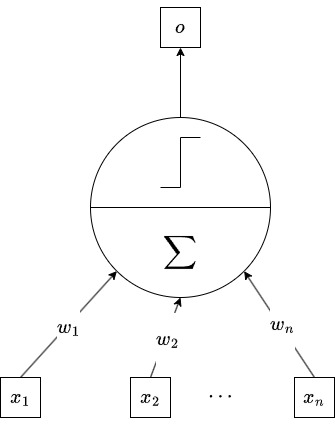
\includegraphics[width=0.5\linewidth]{img/img-perceptron}
			\caption{The perceptron}
			\label{fig:img-perceptron}
		\end{figure}
		
		
		A simple learning algorithm fits a perceptron to any linearly separable set.


		\bigskip
		\subsubsection{Multilayer perceptron}
		
		A multilayer perceptron is made up of fully connected layers. It contains an input layer, a number of hidden layers, and an output layer. This structure allows us to model more complex relationships when compared to the simpler perceptron. 
		
		The building blocks of a perceptron are the following:
		
		\begin{itemize}
			\item Each input feature is connected directly to an input neuron to forward the features into the network.
			\item One, or more than one, hidden layers, each having a designated number of nodes, follow. These layers transform the feature information at each level.
			\item Finally, an output layer consisting of one node (if the task is regression or binary classification) or more nodes (if the task is multi-class classification) gives us the result of the network.
		\end{itemize}
		\bigskip
		
		\begin{figure}[H]
			\centering
			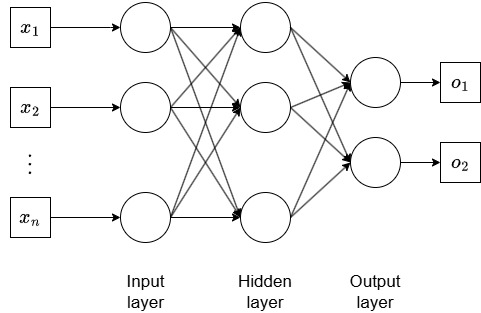
\includegraphics[width=0.7\linewidth]{img/img-multilayer-perceptron}
			\caption{A multilayer perceptron with a single hidden layer}
			\label{fig:img-multilayer-perceptron}
		\end{figure}
		\bigskip
		
		\begin{enumerate}
			\item Forward propagation involves feeding feature information to the input layer, passing it through all hidden layers, and finally to the output layer to generate a predicted output. A linear transformation followed by a non-linear activation generates the output for every node at each layer. Forward propagation is comprised of the following steps:
			
			\bigskip
			\begin{enumerate}
				\item For each neuron in layer $j$, the weighted sum of its inputs is calculated as:
				\begin{equation}
					z_j = \sum_{i=1}^{n_j} w_{ij}^{(j)} x_i^{(j-1)} + b_j
				\end{equation}

				Where:
				\begin{description}
					\item[$x_i^{(j-1)}$] Input from the $i^{th}$ neuron of the previous layer $j-1$.
					\item[$w_{ij}^{(j)}$] Weight connecting the $i^{th}$ neuron of layer $j-1$ to the current neuron in layer $j$.
					\item[$b_j$] Bias term for the neuron in layer $j$.
					\item[$z_j$] Result of the linear transformation at the current neuron in layer $j$.
					\item[$n_j$] Number of inputs (or neurons) in the previous layer $j-1$.
				\end{description}
				\bigskip
							
				\item The result of the weighted sum, $z_j$, is passed through a non-linear activation function:
				$$
				a_j = f(z_j)
				$$
				This introduces non-linearity to the model. A list of some common activation functions can be seen in the Table \ref{tab:activation_functions}.
				
				\begin{table}[H]
					\centering
					\begin{tabular}{|l|c|c|}
						\hline
						\textbf{Function} & \textbf{Equation} & \textbf{Diagram} \\ \hline\hline
						Sigmoid & 
						$\sigma(x) = \frac{1}{1+e^{-x}}$ & 
						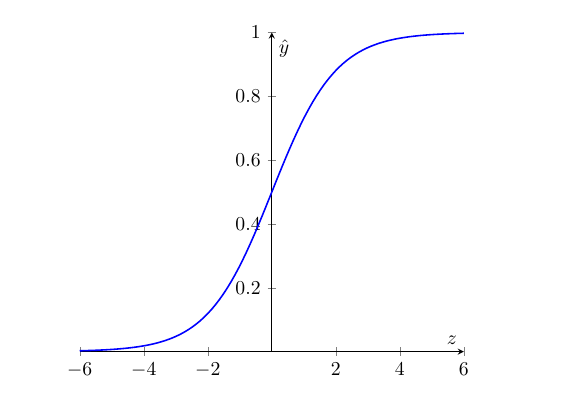
\includegraphics[width=0.3\linewidth]{img/img-neural-network-activation-functions-sigmoid} \\ \hline\\
						
						Tanh & 
						$tanh(x)$ & 
						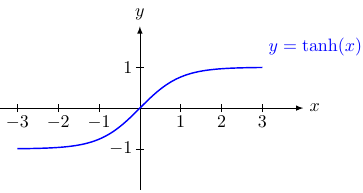
\includegraphics[width=0.3\linewidth]{img/img-neural-network-activation-functions-tanh} \\ \hline \\
						
						Leaky Relu & 
						$max(0.2x, x)$ & 
						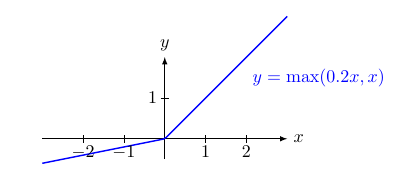
\includegraphics[width=0.3\linewidth]{img/img-neural-network-activation-functions-leaky-relu} \\ \hline \\
						
						Relu & 
						$max(0, x)$ & 
						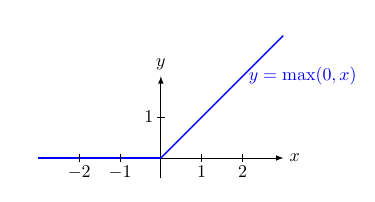
\includegraphics[width=0.3\linewidth]{img/img-neural-network-activation-functions-relu} \\ \hline 
					\end{tabular}
					\caption{Activation Functions}
					\label{tab:activation_functions}
				\end{table}
			\end{enumerate}
			\bigskip

			\item The predicted output is compared to the actual output using a loss function to compute the loss. A loss function measures the difference between the actual target values and the model's predicted results. For a single prediction:
			$$
			\text{Loss}(\hat{y}, y) = f(\hat{y}, y)
			$$
			Where:
			\begin{description}
				\item[$\hat{y}$] Predicted value.
				\item[$y$] Actual value.
				\item[$f$] Specific loss function formula.
			\end{description}
			\bigskip

			The cost function aggregates the loss over the entire dataset:
			$$
			\frac{1}{m} \sum_{i=1}^m \mathcal{L}(\hat{y}, y)
			$$
			
			\bigskip
			Two examples of cost functions are the following:
			\begin{itemize}
				\item Mean Squared Error (MSE):
				\begin{equation}
					\text{MSE} = \frac{\sum_{i=1}^n (\hat{y}^{(i)} - y^{(i)})^2}{n}
				\end{equation}

				
				\item Binary Cross-Entropy:
				Commonly used for binary classification problems:
				\begin{equation}
					L = -\frac{1}{N} \sum_{i=1}^N \left[ y_i \log(\hat{y}_i) + (1 - y_i) \log(1 - \hat{y}_i) \right]
				\end{equation}

				\bigskip
				Where:
				\begin{description}
					\item[$L$] The average loss (cost) across all $N$ samples in the dataset.
					\item[$y_i$] The true label for the $i^{th}$ sample, where $y_i \in \{0, 1\}$.
					\item[$\hat{y}_i$] Predicted probability for $y_i = 1$.
					\item[$1 - \hat{y}_i$] Predicted probability for $y_i = 0$.
					\item[$\log$] The natural logarithm.
				\end{description}
				\bigskip

			\end{itemize}
			\bigskip
			
			\item Backpropagation is the process by which the network's weights and biases are adjusted to minimize loss. The loss is propagated backwards from the output layer to the input layer. At each step, the gradient of the loss with respect to the parameters determines the adjustment. The following steps make up the backpropagation phase:
			
			\bigskip
			\begin{enumerate}
				\item The gradient of the loss with respect to each weight and bias in every node is calculated, starting from the output layer and moving backwards to the input layer.
				\item The gradient for any layer builds on the gradient of the subsequent (later) layers.
				\item The network's parameters for any node are adjusted in the direction opposite to the respective gradient using optimization algorithms like stochastic gradient descent (SGD) or variants such as the Adam optimizer.
			\end{enumerate}
		\end{enumerate}


		\bigskip
		\subsubsection{Stochastic gradient descent}
		
		Stochastic gradient descent is an optimization algorithm that optimizes the parameters $\Theta$ of the network, to minimize the loss
		
		$$
		\Theta = \arg \min_{\Theta}\frac{1}{N} \sum_{i=1}^{n}l(x_i, \Theta)
		$$

		Where:
		\[
		\begin{array}{ll}
			x_{1,2,\dots,N} & \text{The training set.} \\
			l(x_i, \Theta) & \text{The loss for a given data point } x_i. \\
			N & \text{The number of examples in the dataset.}
		\end{array}
		\]
		\bigskip
		
		As Wu noted\cite{wu2017introduction}, the loss, $z$ is a supervision signal that guides any modifications that should take place on the parameters. The stochastic gradient descent method of such modification is as follows:
		
		$$
		\theta^i\leftarrow \theta^i - \eta \frac{\partial z}{\partial \theta^i}
		$$
		where 
		$i$ represents the layer index
		$\eta$ is the learning rate
		$\frac{\partial z}{\partial \theta^i}$ is the gradient of the loss $z$ with respect to parameter $\theta^i$
		
		The parameters are updated iteratively,  as follows:
		
		$$
		\theta^i_{t+1} = \theta^i_{t} - \eta \frac{\partial z}{\partial \theta^i_{t}}
		$$
		
		There are a few considerations that are important to note about stochastic gradient descent.
		
		The learning rate affects the step size for each update, that is how much the parameters are adjusted in the direction of the gradient. A large learning rate might result in overshooting and even divergence, whereas a small learning rate leads to more stable convergence, albeit slower
		
		The parameters are updated for every sample or for a small batch of samples, unlike traditional gradient descent that computes that gradients for the entire dataset. This approach leads to faster updates but is also prone to more noise in the optimization process.
		
		
		
		\bigskip
		\subsubsection{Momentum}
		\label{section:momentum}
		
		Momentum is a technique used in training neural networks to accelerate optimization. This accelerated optimization is achieved by considering also the values of previous gradients for each parameter. Momentum can, in this way, mitigate oscillations in the optimization path and speed up learning.
		
		Momentum acts on the update rule of gradient descent by adding a portion of the update from the previous step to the current step. This approach allows the optimizer to maintain a directional memory, or velocity, effectively smoothing out updates and reducing oscillations.
		
		Momentum is commonly integrated with optimization algorithms like SGD and is a key component of advanced optimizers like Adam optimizer in Section \ref{section:adam}.
		
		The momentum update rule is given by:
		
		$$
		v^i_t = \beta v^i_{t-1} + (1 - \beta)\frac{\partial z}{\partial \theta^i_{t}}
		$$
		$$
		\theta^i_{t+1} = \theta^i_t - \eta v^i_t
		$$
		
		Where:
		\begin{description}
			\item[$v^i_t$] The velocity term at step $t$ for the parameters at index $i$.
			\item[$\beta$] The momentum coefficient (e.g., $0.9$), controlling how much of the previous velocity to retain.
			\item[$\frac{\partial z}{\partial \theta^i_{t}}$] The gradient of the loss function $z$ with respect to parameters $\theta^i$ at step $t$.
			\item[$\eta$] The learning rate.
			\item[$\theta^i_t$] The parameters at layer index $i$ at step $t$.
		\end{description}
		\bigskip

		
		
		A typical value is $\beta = 0.9$, which retains 90\% of the previous velocity. Smaller values result in less "memory" of past updates.  


		\bigskip
		\subsubsection{RMSProp}
		\label{section:RMSProp}
		
		Root Mean Square Propagation (RMSProp) is an adaptive learning rate optimization algorithm designed to improve the training of neural networks. Its main function is to address challenges such as inconsistent or large gradient magnitudes. RMSProp helps stabilize convergence during optimization due to its effectiveness in dealing with noisy gradients.
		
		RMSProp adjusts the learning rate for each parameter based on the average of recent squared gradients. In this way, the optimizer adapts to the scale of the gradients, preventing large updates that could destabilize training.  
		
		The algorithm is similar to [[neural-network-momentum]], but here it introduces a running average of squared gradients to normalize parameter updates.
		
		The RMSProp update rule is given by:
		
		\begin{equation}
			S^i_t = \beta S^i_{t-1} + (1 - \beta) \left( \frac{\partial z}{\partial \theta^i_{t}} \right)^2
		\end{equation}

		
		Where:
		\begin{description}
			\item[$S^i_t$] Exponentially weighted moving average of squared gradients at step $t$ for the parameters at layer index $i$.
			\item[$\beta$] Decay rate for the moving average (commonly set to $0.9$).
			\item[$\left( \frac{\partial z}{\partial \theta^i_{t}} \right)^2$] Gradient of the loss function $z$ with respect to parameters $\theta^i_t$ at step $t$ and layer index $i$.
		\end{description}
		\bigskip
		
		
		The parameters are updated using a learning rate scaled by the square root of $S^i_t$ (with a small value $\epsilon$ added for numerical stability):
		
		\begin{equation}
			\theta^i_{t+1} = \theta^i_t - \frac{\eta}{\sqrt{S_t + \epsilon}} 
			\left( \frac{\partial z}{\partial \theta^i_{t}} \right)
		\end{equation}
		
				
		Where:
		\begin{description}
			\item[$\eta$] Global learning rate, which is set to $0.001$ in most frameworks.
			\item[$\epsilon$] Small constant (e.g., $10^{-8}$) to prevent division by zero.
		\end{description}
		\bigskip

		
		RMSProp is a widely used optimizer that forms the foundation for more advanced methods such as adam optimizer that is discussed in detail in Section \ref{section:adam}. It is especially effective in training deep neural networks where gradient magnitudes can vary significantly.

	
		\bigskip
		\subsubsection{Adam optimizer}
		\label{section:adam}
		
		The Adam Optimizer (Adaptive Moment Estimation) is a widely used optimization algorithm for training deep learning models. It combines the benefits of momentum and rmsprop to provide an efficient, robust, and adaptable optimizer. Adam is particularly effective for problems with sparse gradients and non-stationary objectives.
		
		
		Adam optimizer had a number of hyper parameters:
		
		\begin{itemize}
			\item Learning Rate $\alpha$: \texttt{0.001}
			\item First Moment Decay Rate $\beta_1$: \texttt{0.9}
			\item Second Moment Decay Rate $\beta_2$: \texttt{0.999}
			\item Numerical Stability Term $\epsilon$: \texttt{1e-8}
		\end{itemize}
		\bigskip

		
		The Adam-optimizer update rule is given by the following steps:
		\bigskip
		\begin{enumerate}
			\item First, calculate the first moment estimate, or the Momentum that we discussed in Section \ref{section:momentum}, which is the exponentially weighted moving average of the gradients. This is done to smooth gradient updates over time by including past gradients and thus maintaining a directional memory:
			$$
			m^i_t = \beta_1 m^i_{t-1} + (1 - \beta_1)\frac{\partial z}{\partial \theta^i_{t}}
			$$
			
			\item Calculate the second moment estimate, which is the basic idea of RMSProp that we discussed in Section \ref{section:RMSProp}, to track the exponentially weighted variance of gradients:
			$$
			v^i_t = \beta_2 v^i_{t-1} + (1 - \beta_2) \left( \frac{\partial z}{\partial \theta^i_{t}} \right)^2
			$$
			
			\item Correct these results for initialization bias:
			$$
			\hat{m}^i_t = \frac{m^i_t}{1 - \beta_1^t}
			$$
			$$
			\hat{v}^i_t = \frac{v^i_t}{1 - \beta_2^t}
			$$
			
			\item Update the parameters using the corrected estimates:
			$$
			\theta^i_{t+1} = \theta^i_t - \frac{\alpha \hat{m}^i_t}{\sqrt{\hat{v}^i_t} + \epsilon}
			$$
		\end{enumerate}


		\bigskip
		\subsubsection{Batch normalization}
		
		Batch normalization is used to control the statistics of the activations in the neural networks. It is commonly used in neural network architectures, and it is usually found after layers that have multiplications, like linear or convolutional layers 
		
		Let us consider a hidden state neural net node
		
		We have basically a pre-activation value, that is the result of 
		
		$$
		z = \left(\sum_{i=1}^{n} x_i w_i \right)+ b
		$$
		
		That is fed into a non-linear element such as RELu or tanh.
		
		\begin{itemize}
			\item We do not want the pre-activation to be very small as the tanh activation will not effectively activate.
			\item We also do not want these values to be too large, as the tanh will become saturated.
			\item Furthermore, we want these values to be roughly Gaussian, that is, with a mean of 0 and a standard deviation of 1.
		\end{itemize}
		\bigskip
		
		Sergey Ioffe and Christian Szegedy propose batch-normalization \cite{ioffe2015batch} to take the hidden states and normalize them to be Gaussian.
		
		\begin{figure}
			\centering
			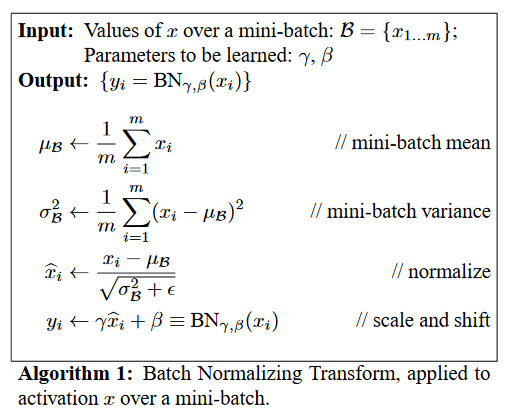
\includegraphics[width=0.7\linewidth]{img/img-ioffeBatchNormalizationAccelerating2015-1}
			\caption{Batch normalization algorithm, from \cite{ioffe2015batch}}
			\label{fig:img-ioffebatchnormalizationaccelerating2015-1}
		\end{figure}
		

		
		There are two ways whereby batch normalization can be implemented:
		
		\begin{itemize}
			\item Pre-activation normalization, where batch-normalization is carried out before the activation function is applied.
			\item Post-activation normalization, where batch-normalization is carried out after the activation function is applied.
		\end{itemize}
		\bigskip
		
		The original paper specified pre-activation normalization, however studies have shown that post-activation batch normalization will give superior results.



		\bigskip
		\subsubsection{Regularization}
		
		Regularization are techniques used to prevent overfitting in machine learning. This is achieved by adding a penalty term to the [[loss-function]], that discourage the model from assigning larger weights to features.
		
		L1 regularization or Lasso Regularization adds the sum of the absolute values of the weights to the [[loss-function]]:
		
		\begin{equation}
			\mathcal{L}_{L1} = \mathcal{L} + \lambda \sum_{i=1}^n |w_i|
		\end{equation}

		
		Where:
		\begin{description}
			\item[$\mathcal{L}$] The original loss function (e.g., cost-function-mean-square-error, cost-function-cross-entropy).
			\item[$\lambda$] The regularization strength, a hyperparameter.
			\item[$w_i$] The weight of the $i^{th}$ node.
		\end{description}
		\bigskip
		
		L1 regularization drives some weights to zero, thus encouraging sparsity in the network. Since L1 penalizes large weights, it promotes simpler networks with improved generalization.
		
		L2 or Ridge regularization adds the sum of the squared values of the weights to the [[loss-function]]:
		

		\begin{equation}
			\mathcal{L}_{L2} = \mathcal{L} + \lambda \sum_{i=1}^n w_i^2
		\end{equation}
		
		Where:
		\begin{description}
			\item[$\mathcal{L}$] The original loss function (e.g., cost-function-mean-square-error, cost-function-cross-entropy).
			\item[$\lambda$] The regularization strength, a hyperparameter.
			\item[$w_i$] The weight of the $i^{th}$ node.
		\end{description}
		\bigskip
		
		
		L2 penalizes large weights but does not drive them to zero but shrinks them closer to zero. It hence promotes smoother solutions and avoids sharp changes in parameter values.



	%% logistic regression
	%% -------------------

	\bigskip
	\subsection{Machine learning technique - Logistic regression}

		
		Logistic regression is a machine learning algorithm commonly used for binary classification tasks.
		
		Given a feature vector $X \in \mathbb{R}^{n_x}$, the goal of logistic regression is to predict the probability $\hat{y}$ that a binary output variable $y$ takes the value 1, given $X$, that is $\hat{y} = P(y=1|X)$, $0\le y\le1$. 
		For example, in the case of image classification, logistic regression can be used to predict the probability that an image contains a cat.
		
		\begin{figure}[H]
			\centering
				\begin{tikzpicture}
		\usetikzlibrary{calc}
		% Draw the ellipse
		\draw  (-0,0) circle (2);
		% Node at the center of the ellipse
		\node[circle, inner sep=0pt] (v2) at (-0,0) {};
		% Nodes for the lines
		\node (v1) at (-5, 2) {$x_1$};
		\node (v3) at (-5,0) {$x_2$};
		\node (v4) at (-5,-2) {$x_n$};
		\node (v7) at (4,0) {$\hat{y}$};
		% Draw lines stopping at the ellipse
		\draw[-] (v1) -- ($(v2)!0.37!(v1)$);
		\draw[-] (v3) -- ($(v2)!0.4!(v3)$);
		\draw[-] (v4) -- ($(v2)!0.37!(v4)$);
		\draw[-] (v7) -- ($(v2)!0.5!(v7)$);
		\node (v5) at (0,2) {};
		\node (v6) at (0,-2) {};
		\draw  (v5) edge (v6);
		\node [font=\tiny] at (-1,0) {$z=\textbf{W}^T\textbf{X}+b$};
		\node [font=\tiny] (v8) at (1,0) {$\hat{y}=\sigma(z)$};
		\node at (-3,1.5) {$w_1$};
		\node at (-3,0.25) {$w_2$};
		\node at (-3,-1.5) {$w_n$};
		\node at (-3,-0.5) {$\vdots$};
\end{tikzpicture}

			\caption{A logistic regression model}
			\label{fig:logisticregression}
		\end{figure}
		
		
		Logistic regression can be visualized as the model shown in Figure \ref{fig:logisticregression}. It consists of several main components:
		
		\begin{itemize}[]
			\item Inputs. The input vector to the model $\textbf{X} \in \mathbb{R}^{n_x}$.
			
			\item Parameters. A weight vector $\textbf{W} \in \mathbb{R}^{n_x}$ and a bias term $b \in \mathbb{R}$.  These will form the coefficients of a linear equation that gives the log odds ratio.
			
			\item Pre-activation result: The result is obtained by multiplying the transpose of the weights with the inputs and then adding the bias. 
			\begin{equation}
				z = \textbf{W}^{T}\textbf{X} + b = 
				\begin{bmatrix} 
					w_1 & w_2 & \dots & w_n
				\end{bmatrix}
				\begin{bmatrix} 
					x_1 \\ 
					x_2 \\ 
					\vdots \\ 
					x_n
				\end{bmatrix} + b
			\end{equation}

			
			
			\item Sigmoid function. A function as shown in Figure \ref{fig:sigmoid}, $\sigma(z) = \frac{1}{1 + e^{-z}}$, which maps any real number $z$ to the range $(0,1)$. This function is used to ensure that the predicted probability $\hat{y}$ is always between 0 and 1.
			
			\begin{figure}[H]
				\centering
				 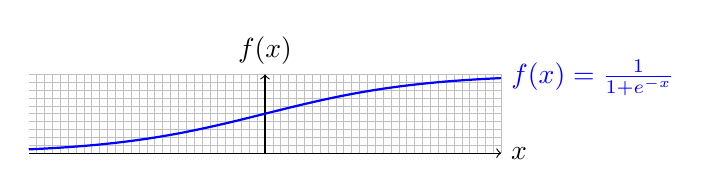
\begin{tikzpicture}[domain=-3:3] [H]% Reduced domain for a narrower plot
	% Grid and axes
	\draw[very thin,color=lightgray, step=0.1] (-3,-0) grid (3,1);
	\draw[->] (-3,0) -- (3,0) node[right] {$x$};
	\draw[->] (0,-0) -- (0,1) node[above] {$f(x)$};
	
	% Sigmoid function
	\draw[color=blue, thick, samples=100] 
	plot (\x, {1/(1 + exp(-\x))}) 
	node[right] {$f(x) = \frac{1}{1 + e^{-x}}$};
\end{tikzpicture}

				\caption{Sigmoid activation function}
				\label{fig:sigmoid}
			\end{figure}
			
			\item Output. The predicted probability $\hat{y}$ is computed as $\hat{y} = \sigma(z) = \sigma(\textbf{W}^{T}\textbf{X} + b)$.
		\end{itemize}
		\bigskip
		
		
		A term that is often encountered in this scenario is the log-odds ratio or logit. Logistic regression models the probability $P(y = 1 \mid X)$, of the binary dependent variable $Y$ given the predictor variables $\textbf{X} = \{x_1, x_2, \dots, x_n\}$. The goal is to find a relationship between $P(y=1)$, and the predictors $\textbf{X}$.
		
		The probability is modelled using the sigmoid function:
		$$P(y = 1 \mid X) = \frac{1}{1 + e^{-\eta}}$$
		
		Where:
		$\eta = b + w_1 x_1 + w_2 x_2 + \dots + w_n x_n$  is the linear regression function
		
		The odds of $y=1$ are defined as the ratio of the probability of success to the probability of failure:
		
		$$\text{Odds} = \frac{P(y = 1)}{1 - P(y = 1)}$$
		
		Taking the natural logarithm of the odds gives the 
		[log-odds-ratio]] or logit:
		
		$$\text{Log-Odds} = \ln\left(\frac{P(y = 1)}{1 - P(y = 1)}\right)$$
		
		From the sigmoid function, we can derive the relationship between the probability and the log-odds-ratio:
		
		$$P(y = 1) = \frac{1}{1 + e^{-\eta}}$$
		$$1 - P(y = 1) = 1 - \frac{1}{1 + e^{-\eta}} = \frac{e^{-\eta}}{1 + e^{-\eta}}$$
		
		The odds, therefore, are
		$$\text{Odds} = \frac{P(y = 1)}{1 - P(y = 1)} = \frac{\frac{1}{1 + e^{-\eta}}}{\frac{e^{-\eta}}{1 + e^{-\eta}}} = e^{\eta}$$
		
		
		Taking the natural logarithm of both sides gives the log-odds:
		
		$$ln\left(\frac{P(y = 1)}{1 - P(y = 1)}\right) = \eta$$
		
		Substituting $\eta = b + w_1 x_1 + w_2 x_2 + \dots + w_n x_n$
		
		\begin{equation}
			\ln\left(\frac{P(y = 1)}{1 - P(y = 1)}\right) = \eta = b + w_1 x_1 + w_2 x_2 + \dots + w_n x_n
		\end{equation}
		
		\bigskip
		
		We conclude this overview of logistic regression by looking at how they work and learn.	The weight vector $\textbf{W}$ and the bias term $b$ are learned from a labelled training set by minimizing a suitable loss function using techniques such as gradient descent or its variants. Once trained, the logistic regression model can be used to predict the probability of the binary output variable for new input examples.
		
		
		The feedforward process for logistic regression can be described as follows:
		
		\begin{enumerate}[]
			\item Compute $z$ as the dot product of the weight vector $\textbf{W}$ and the input features, plus the bias term $b$, transforming the input features info a single scalar $z$ that represents the log-odds of the output being $y=1$: 
			\begin{equation}
				z= \textbf{W}^{T}\textbf{X} + b
			\end{equation}
			
			\item Pass $z$ through the sigmoid function to map the log-odds $z$ to a probability $\hat{y} = P(y = 1 \mid X)$, ensuring the output is between 0 and 1: 
			\begin{equation}
				\hat{y} = \sigma(z) = \frac{1}{1 + e^{-z}}
			\end{equation}
			
			\item During training, we define the loss function $\mathcal{L}$ as the negative log-likelihood of the predicted output given the true label: 
			\begin{equation}
				\mathcal{L} = -\left(y\ln(\hat{y}) + (1-y)\ln(1-\hat{y})\right)
			\end{equation}
		\end{enumerate}
		
		For a trained system, we compare $\hat{y}$ to a threshold to convert the probabilistic output into the final binary classification.
		
		\bigskip
		
		We now look at \textbf{feedback process} for logistic regression. To optimize the weight vector $\textbf{W}$, we compute the derivatives of the loss function with respect to each weight and the bias term and use these derivatives to update the weights in the opposite direction of the gradient. This is known as gradient descent.
		
		To compute the derivatives, we use the chain rule:
		
		$$
		\frac{\partial\mathcal{L}}{\partial w_i} =
		\frac{\partial\mathcal{L}}{\partial \hat{y}} \cdot
		\frac{\partial \hat{y}}{\partial z} \cdot
		\frac{\partial z}{\partial w_i}
		$$ and
		$$
		\frac{\partial\mathcal{L}}{\partial b} =
		\frac{\partial\mathcal{L}}{\partial \hat{y}} \cdot
		\frac{\partial \hat{y}}{\partial z} \cdot
		\frac{\partial z}{\partial b}
		$$
		
		We can then use these derivatives to update the weights as follows:
		
		
		\begin{equation}
			w_i \leftarrow w_i - \alpha \frac{\partial \mathcal{L}}{\partial w_i}
		\end{equation}
		
		and
		
		\begin{equation}
			b \leftarrow b - \alpha \frac{\partial \mathcal{L}}{\partial b}
		\end{equation}
		
		
		Where $\alpha$ is the learning rate, which controls the step size of the updates. By iteratively performing these updates on a training set, we can find the optimal weight vector $\textbf{W}$ that minimizes the loss function on the training set.
		
		\bigskip
		
		To calculate the derivatives, let us begin by computing the derivative of the loss function with respect to the predicted output $\hat{y}$:
		
		
		$$
		\frac{\partial \mathcal{L}}{\partial\hat{y}} = 
		\frac{\partial}{\partial\hat{y}} 
		\left(  
		-\left(y\ln(\hat{y}) + (1-y)\ln(1-\hat{y})\right)
		\right) 
		$$
		since 
		$$\frac{d \space (ln (x))}{dx}  = \frac{1}{x}$$we get:
		$$\frac{\partial \mathcal{L}}{\partial \hat{y}} = - \left( \frac{y}{\hat{y}} - \frac{1-y}{1-\hat{y}} \right) $$
		
		The derivative of the predicted output $\hat{y}$ with respect to $z$ is solved using the quotient rule, that is 
		$$
		\frac{d}{dx} \left( \frac{f(x)}{g(x)} \right) = \frac{f'(x)g(x) - g'(x)f(x)}{g^2(x)}
		$$
		
		So, if we let
		
		\begin{table}[!ht]
			\centering
			\begin{tabular}{|l|l|l|}
				\hline
				$f(z) = 1$ & $f'(z) = 0$ \\ \hline
				$g(z)=1 +e^{-z}$ & $g'(z)= -e^{-z}$ \\ \hline
			\end{tabular}
		\end{table}
		
		
		\begin{align*}
			\frac{\partial\hat{y}}{\partial z} 
			& = \frac{\partial}{\partial z} \left( \frac{1}{1 + e^{-z}} \right) \\
			& = \frac{e^{-z}}{(1 + e^{-z})^2} \\
			& = \frac{1}{(1 + e^{-z})} \space \frac{e^{-z}}{(1 + e^{-z})} \\
			& = \frac{1}{(1 + e^{-z})} \space \frac{1 + e^{-z} -1}{1 + e^{-z}} \\
			& = \frac{1}{(1 + e^{-z})} \space \left( \frac{1 + e^{-z}}{1 + e^{-z}} - \frac{1}{1 + e^{-z}} \right)\\
			& = \hat{y}(1-\hat{y})\\
		\end{align*}
		
		
		
		The derivative of $z$ with respect to $w_i$:
		
		\begin{equation}
			\begin{split}
				\frac{\partial z}{\partial w_i} 
				&=	\frac{\partial}{\partial w_i} \textbf{W}^T \textbf{X} + b\\
				&= 	\frac{\partial}{\partial w_i} (w_1 x_1 + \dots + w_ix_i+\dots+w_nx_n + b)\\
				&= x_i\\
			\end{split}
		\end{equation}
		
		Similarly,
		
		
		\begin{equation}
			\begin{split}
				\frac{\partial z}{\partial b} 
				&= \frac{\partial}{\partial b} \textbf{W}^T \textbf{X} + b\\
				&= 	\frac{\partial}{\partial b} (w_1 x_1 + \dots + w_ix_i+\dots+w_nx_n + b)\\
				&= 1\\
			\end{split}	
		\end{equation}	
		
		Therefore
		
		
		\begin{align*}
			\frac{\partial\mathcal{L}}{\partial w_i} 
			&= \frac{\partial\mathcal{L}}{\partial \hat{y}} \cdot
			\frac{\partial \hat{y}}{\partial z} \cdot
			\frac{\partial z}{\partial w_i} \\
			& = 
			-\left(
			\frac{y}{\hat{y}} - \frac{1-y}{1-\hat{y}}
			\right) \cdot
			\hat{y}(1-\hat{y})
			\cdot
			x_i\\
			&= 
			-\left(
			\frac{-y(1-\hat{y}) + (1-y)\hat{y}}{\hat{y}(1-\hat{y})}
			\right) \cdot
			\hat{y}(1-\hat{y})
			\cdot
			x_i\\
			&= \left[ (1-y)\hat{y} -y(1-\hat{y})  \right]x_i\\
			&= \left[ \hat{y} -y\hat{y} -y +y\hat{y}\right]x_i\\
		\end{align*}
		\begin{equation}
			\frac{\partial\mathcal{L}}{\partial w_i} = (\hat{y} - y) x_i
		\end{equation}
		
		and similarly
		
		\begin{equation}
			\frac{\partial\mathcal{L}}{\partial b} =
			\left(
			\hat{y} - y
			\right)
		\end{equation}
		

	%% knn
	%% ---
	
	\bigskip
	\subsection{Machine learning technique - K-nearest neighbours algorithm}
	
	K-nearest neighbours is simple yet robust for datasets with well-structured local relationships. It is particularly effective for non-linear decision boundaries and finds applications in anomaly detection, pattern recognition, and recommendation systems.
	
	The k-nearest neighbours algorithm is non-parametric, that is, it does not make assumptions about the underlying distribution or functional form of the data; instance-based, that is, it does not explicitly learn a model during a training phase, but it relies on the raw training data to make predictions at query time, unlike parametric models, which "learn" a set of fixed parameters (e.g., coefficients in linear regression) during training,   learning method used for classification and regression tasks. It predicts the output of a query point based on the labels or values of its $k$-nearest neighbours in feature space.
	
	KNN does not assume a specific functional form for the data. Instead, it relies on the local structure of the dataset. For a given query point $x$, the algorithm uses a distance metric to identify its $k$-nearest neighbours and infers the prediction by aggregating their outcomes. Typical distance metrics include:
	\begin{enumerate}
		\item Euclidean Distance
		$$
		d(x, x') = \sqrt{\sum_{i=1}^{n} (x_i - x'_i)^2}
		$$
		
		\item Manhattan Distance
		$$
		d(x, x') = \sum_{i=1}^{n} |x_i - x'_i|
		$$
		
		\item Minkowski Distance. Note that for $p = 2$, this reduces to the Euclidean distance; for $p = 1$, it becomes the Manhattan distance.
			$$
			d(x, x') = \left( \sum_{i=1}^{n} |x_i - x'_i|^p \right)^{1/p}
			$$
		\end{enumerate}
		
		
		In classification tasks, the predicted class  $\hat{y}$ for a query point $x$ is determined by majority voting among its  $k$-nearest neighbours. If we let $N_k(x)$ represent the set of the $k$-nearest neighbours,he predicted class is given by:
		
		$$
		\hat{y} = \text{argmax}_c \sum_{x' \in N_k(x)} \mathbb{I}(y(x') = c)
		$$
		
		Where:
		$$
		\begin{array}{ll}
			\text{argmax}_c & \parbox[t]{0.4\textwidth}{Identifies the class $c$ with the highest count among the neighbours.} \\
			\mathbb{I}(\cdot) & \parbox[t]{0.4\textwidth}{The indicator function, which equals  1 if  $y(x') = c$,  and 0 otherwise.}
		\end{array}
		$$

		
		The parameter $k$ determines the number of neighbours considered.
		
		\begin{itemize}
			\item A small $k$ (e.g., $k = 1$) makes the model sensitive to noise, as predictions rely heavily on individual points.
			\item A large $k$ smooths the decision boundary but may lead to underfitting.
		\end{itemize}
				
		Finding the optimal value for $k$ is one of the main challenges in the k-nearest neighbour. Cross-validation is typically employed to find a value using the following procedure:
		
		\bigskip
		\begin{enumerate}
			\item Iterate Over Candidate Values of $k$
			\begin{itemize}
				\item Choose a range of potential $k$ values, for example, $k = 1, 2, \dots, 20$.
			\end{itemize}
			
			\item Evaluate Performance for Each $k$
			\begin{itemize}
				\item For each $k$, use $K$-fold cross-validation:
				\begin{itemize}
					\item Train the KNN model using $K-1$ folds.
					\item Validate it on the remaining fold.
					\item Compute the average performance metric across all $K$ folds.
				\end{itemize}
			\end{itemize}
			
			\item Select $k$ with the Best Performance
			\begin{itemize}
				\item After evaluating all $k$ values, choose the $k$ that maximizes the performance metric (e.g., accuracy) or minimizes the error.
			\end{itemize}
		\end{enumerate}
		\bigskip
		
		The $k$-nearest neighbour algorithm is, therefore, as follows;
		
		\bigskip
		\subsubsection{Input}
		\begin{itemize}
			\item Dataset: $D = \{(x_1, y_1), (x_2, y_2), \dots, (x_N, y_N)\}$, where $x_i$ is the feature vector, and $y_i$ is the corresponding label or value.
			\item Query point: $x_{query}$, the data point for which the prediction is required.
			\item Number of neighbours: $k$, the number of nearest neighbours to consider.
			\item Distance metric: $d(x, x')$ (e.g., Euclidean distance).
		\end{itemize}
		
		\subsubsection{Steps:}
			\begin{enumerate}
			
			\item Calculate Distance. For the query point $x_{query}$, compute the distance to every point $x_i$ in the dataset $D$ using the chosen distance metric. For Euclidean distance:
			$$
			d(x_{query}, x_i) = \sqrt{\sum_{j=1}^{n} (x_{query_j} - x_{i_j})^2},
			$$
			$$
			\quad \forall i \in \{1, 2, \dots, N\}.
			$$
			
			\item Sort Neighbours. Rank all data points $x_i$ in $D$ by their distance to $x_{query}$ in ascending order. Let this sorted set be $D_{sorted}$.
			
			\item Select $k$-Nearest Neighbours. Extract the top $k$ data points from $D_{sorted}$. Denote this set as $N_k(x_{query})$.
			
			\item Aggregate Neighbours' Outputs.
			\begin{itemize}
				\item For \textbf{classification}: Perform majority voting among the labels $y_i$ of the $k$-nearest neighbours:
				$$
				\hat{y} = \text{argmax}_c \sum_{x_i \in N_k(x_{query})} \mathbb{I}(y_i = c),
				$$
				where $\mathbb{I}(y_i = c)$ is an indicator function that equals $1$ if $y_i = c$, and $0$ otherwise.
				
				
			\end{itemize}
			
			\item \textbf{Output Prediction:}
			Return $\hat{y}$ as the predicted label (for classification) or value (for regression) for $x_{query}$.
			
		\end{enumerate}
		
		\subsubsection{Output:}
		The predicted label or value $\hat{y}$ for the query point $x_{query}$.
		


	% rescaling and optimization
	% --------------------------

	\subsection{Feature scaling}

		Feature scaling is an important data transformation process. It is a very important aspect of many machine learning algorithms including logistic regression, support vector machines and neural networks, as, the performance of such algorithms is adversely impacted when the numerical features have different scales. The two methods to transform features on the same scale are normalization and rescaling.
		
		During normalization or rescaling, values are scaled and shifted so that they are mapped onto the $[0,\space 1]$ interval. This is achieved by applying the following transformation;
		$$
		x_{normalized} = \frac{x - x_{min}}{x_{max}-x_{min}}
		$$
		Normalization is also sometimes referred to as min-max scaling.
		
		Standardization is particularly suited for algorithms that assume Gaussian distributions, like linear regression and logistic regression. It is achieved by first subtracting values from the mean so that the mean of the normalized values is zero, and then dividing by the standard deviation so that the variance of the normalized distribution is one. Thus;
		$$
		x_{standardized} = \frac{x - \mu}{\sigma}
		$$
		Unlike normalization, the range of standardization is not fixed, and this can sometimes be an issue if a value in the $[0,\space 1]$ interval is expected.  Standardization is however more resilient to the effect of outliers.
		
		Tree based machine learning models, like decision trees and random forests do not normally require feature scaling.


	% cross validation
	% ----------------
	
	\subsection{Cross-validation}
	
		Cross-validation is a technique that can be applied to any ML algorithm that is aimed to reduce overfitting by estimating how well each hypothesis generalizes to unseen data. In practice, a portion of the data is reserved for this purpose.
		
		The $K$-fold cross validation technique splits the dataset into $k$ folds, training that model on $k-1$ folds and testing on the remaining one. The test fold is rotated and the process is repeated so that each fold will act as the test set once. Metrics like mean square error are averaged across folds, ensuring a robust estimate.
		
		Therefore, if for example, we split the data into 10 folds, so that each fold will have $n/10$ records, we train the model on 9 folds and test on the remaining one. We then rotate the test fold and repeat this process 10 times. The final performance metric is computed as the mean of the metrics across the 10 folds.
		
		In stratified $K$-fold cross validation, the folds have the same proportion of the classes as in the original dataset.
		
		Other types of cross validation include Leave one out cross-validation, where each data point is used as a test set once.
	
	
	% dimentionality reduction 
	% ------------------------
	
	
	% feature selection
	% -----------------
	
	
	\subsection{Feature Selection}
	
	Feature selection identifies and retains the most relevant features in a dataset to improve model performance and reduce complexity. It involves reducing the dimensionality of the original problem by selecting a subset of features. For example:
	
	$$
	\begin{array}{c}
		\text{Original problem (with } n \text{ dimensions):} \\
		\text{A facial image represented by } 32 \text{ facial action units.}
	\end{array}
	\quad \longrightarrow \quad
	\begin{array}{c}
		\text{Reduced problem (with } k < n \text{ dimensions):} \\
		\text{A facial image represented by } 12 \text{ facial action units.}
	\end{array}
	$$
	
	In feature selection, $k$ features are selected out of $N$ to minimize the learner error. This process can be mathematically represented as:
	
	$$
	\begin{bmatrix} 
		x_1 \\ x_2 \\ \vdots \\ x_N 
	\end{bmatrix} 
	\quad
	\xrightarrow{\text{Feature Selection}} 
	\quad 
	\begin{bmatrix} 
		x_{i_1} \\ x_{i_2} \\ \vdots \\ x_{i_k} 
	\end{bmatrix}.
	$$
	
	Feature selection is essential for several reasons:
	\begin{itemize}
		\item Curse of Dimensionality. High-dimensional datasets often lead to models requiring more data and computation and are prone to poor generalization.
		\item Overfitting. Excessive features can cause a model to fit noise in the data, leading to overfitting.
		\item Visualization. Reduced dimensionality makes it possible to visualize data in two or three dimensions.
	\end{itemize}
	
	
	Filter-based feature selection is a method that selects features based on statistical measures of their relevance to the target variable, independently of any machine learning model.
	
	Filter-based feature selection has two primary aims:
	\begin{enumerate}
		\item Select features that are independent of each other, ensuring that each feature contributes new information.
		\item Select features that are highly dependent on the target variable, avoiding features that do not improve model performance.
	\end{enumerate}
	
	Types of filter-based feature selection methods include:
	\begin{itemize}
		\item For small numbers of features:
		\begin{itemize}
			\item Use scatterplots to visually assess relationships between features and the target variable.
		\end{itemize}
		\item For analyzing relationships:
		\begin{itemize}
			\item Use Pearson correlation to measure the linear correlation between features and the target variable.
			
		The Pearson correlation is a normalized version of covariance\cite{penny2008mathematics} and measures the degree of linear correlation between two variables.
			
			
			\begin{align*}
				r &= \frac{\sigma_{xy}}{\sigma_x\sigma_y}\\
				  &= \frac{\sum (X_i - \bar{X})(Y_i - \bar{Y}) }{\sqrt{\sum (X_i - \bar{X})^2 \sum (Y_i - \bar{Y})^2}}
			\end{align*}
			
			
			
			where:
			\begin{description}
				\item[$X_i$, $Y_i$:] The individual data points.
				\item[$\bar{X}$, $\bar{Y}$:] The means of the variables $X$ and $Y$.
			\end{description}
			
			$r$ is unitless, meaning it has no associated units of measurement.
			
			
		\end{itemize}
	\end{itemize}
	
	
	
	
	% quantitative measurements
	% -------------------------
	
	\subsection{Measurement}
	
		Quantitative measurements numerically represent attributes and are fundamental for evaluating machine learning models by providing an objective means to assess the model's performance. We can analyse the model's effectiveness by comparing model predictions to actual outcomes. Appropriate selection and reporting of measurement methods, including their reliability, validity, and potential biases, are essential to ensure accurate interpretation and meaningful results. This section will look at the measurements used in this study.
		
		The function used in machine learning and statistical modelling to quantify the difference between the predicted outputs of a model and the actual target values is called the loss function. It serves as a measure of the model's performance, guiding the optimisation process to improve predictions.
		
		For a single prediction:
		
		$$\text{Loss}(\hat{y}, y) = f(\hat{y}, y)$$
		Where:
		
		
		\begin{compactitem}
			\item [$\hat{y}$]: Predicted value.
			\item [$y$]: Actual value.
			\item [$f$]: Specific loss function formula
		\end{compactitem}
		
		\bigskip
		
		The aggregation of the loss function across the entire dataset is called the cost function so that;
		
		$$
		\text{Cost}(\hat{y}, y) = \frac{1}{N}\sum_{i=1}^{N} \mathcal{L}(\widehat{y}_i, y_i)
		$$
		
		In the problem we are considering, we will try to predict whether a person will recidivate given information about his or her previous criminal history is a binary classifier problem. A binary classifier is a function that can be applied to features $X$ such as $(x_1, x_2, x_3, \dots, x_n)$ and maps them to an output $Y$, where $Y \in \{0, 1\}$. It is a supervised learning technique; therefore, a test set is extracted from the available data to validate the model before being deployed in production.
		
		$$ f(x_1, x_2, x_3, \dots, x_n) = Y \in \{0, 1\}  $$
		
		The function will return a value between 0 and 1; therefore, a threshold value is operated to classify the result as true or false. The model will subsequently classify predictions as true or false according to the threshold value.
		
		
		For the classification problem that we have in hand, we will  primarily use the log-likelihood  cost function defined as:
		
		$$\mathcal{L}_{\text{log-likelihood}} = - \sum_{i=1}^N \left[ y_i \ln(\hat{y}_i) + (1 - y_i) \ln(1 - \hat{y}_i) \right]$$
		
		Negative log-likelihood focuses on the distance between the labels $y_i$ and the predicted probabilities $\hat{y}_i$. If we consider a sample where:
		
		\begin{itemize}
			\item $y_i$ is one and $\hat{y}_i$ is close to 1: $y_i \ln(\hat{y}_i)$ is close to zero, while $(1 - y_i) \ln(1 - \hat{y}_i)$ is zero, so that the resultant loss is close to zero.
			\item $y_i$ is 1 and $\hat{y}_i$ is far from 1: $y_i \ln(\hat{y}_i)$ is large, while $(1 - y_i) \ln(1 - \hat{y}_i)$ is zero so that the resultant loss is large.
			\item $y_i$ is zero and $\hat{y}_i$ is close to 0: $y_i \ln(\hat{y}_i)$ is zero, while $(1 - y_i) \ln(1 - \hat{y}_i)$ is also close to zero so that the resultant loss is close to zero.
			\item $y_i$ is zero and $\hat{y}_i$ is far from 0: $y_i \ln(\hat{y}_i)$ is zero, while $(1 - y_i) \ln(1 - \hat{y}_i)$ is large so that the resultant loss is large.
		\end{itemize}
		\bigskip
		
		In this scenario,  we can obtain four kinds of results:
		
		\begin{table}[!ht]
			\centering
			\begin{tabular}{|l|l|l|p{2cm}|}
				\hline
				Prediction & Classif & Outcome & Description \\ \hline\hline
				1 & 1 & True Positive (TP) & The model correctly predicted the positive class. \\ \hline
				1 & 0 & False Positive (FP) & The model incorrectly predicted the positive class (a false alarm). \\ \hline
				0 & 1 & False Negative (FN) & The model incorrectly predicted the negative class (a miss). \\ \hline
				0 & 0 & True Negative (TN) & The model correctly predicted the negative class. \\ \hline
			\end{tabular}
		\end{table}
		
		The number of samples that are TP, TN, FP or FN can be organised in what is known as a confusion matrix, that is shown in Figure \ref{fig:confusionmatrix}. This tool makes it easy to perform calculations that determine the validity of the model at hand.
		
		\begin{figure}[H]
			\centering
			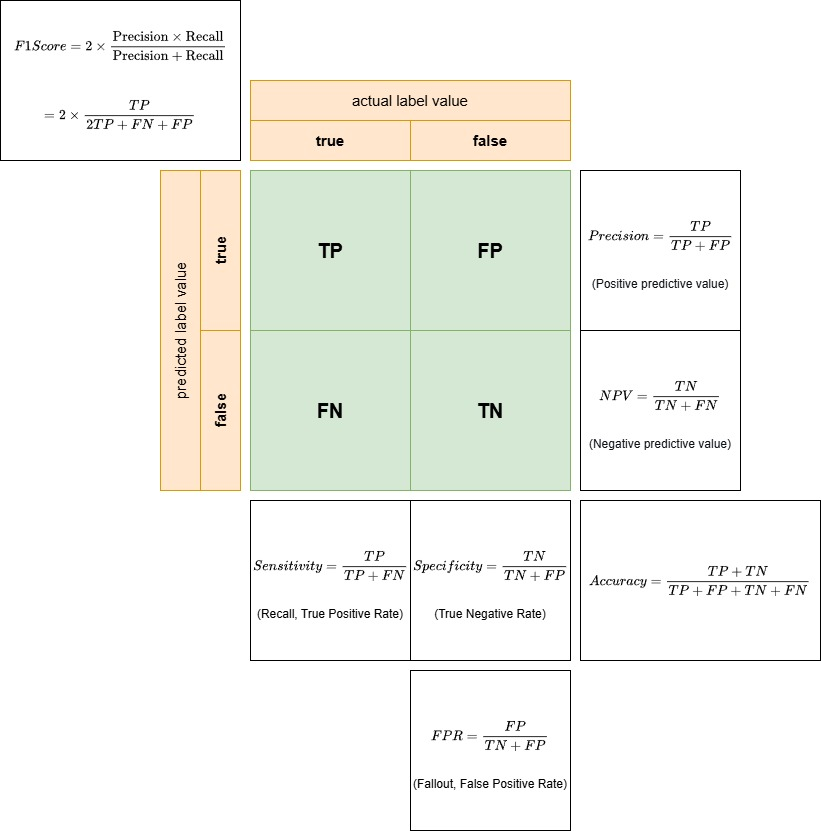
\includegraphics[width=0.9\linewidth]{img/confusion_matrix}
			\caption{Confusion matrix and associated equations}
			\label{fig:confusionmatrix}
		\end{figure}
		
		
		There are several key performance metrics derived from the confusion matrix, each offering a different perspective on evaluating the effectiveness of a binary classification model.
		
		\bigskip
		
		The \textbf{accuracy} of a model is a straightforward measure that evaluates the proportion of correct predictions (both True Positives and True Negatives) out of the total number of predictions. It can be mathematically defined as:
		
		
		$$Accuracy=\frac{TP+TN}{TP+FP+TN+FN}$$
		
		for a dataset,
		$$
		Accuracy = \frac{1}{N} \sum_{i=1}^{N} 1(\hat{y}_i = y_i)
		$$
		
		
		\textbf{Precision} answers the question: "Out of all the observations predicted to be positive, how many were positive?" In other words, it measures the model's ability to avoid false positives.
		
		$$Precision=\frac{TP}{TP+FP}$$
		
		
		\textbf{Recall} or \textbf{sensitivity} measures the model's ability to correctly identify positive cases. It answers the question: "Out of all the actual positive instances, how many did the model correctly identify as positive?"
		
		
		$$Recall=\frac{TP}{TP + FN}$$
		
		\textbf{Specificity} measures the model's ability to identify negative cases correctly. It answers the question: "Out of all the actual negative instances, how many did the model correctly identify as negative?"
		
		The formula for specificity is:
		
		$$Specificity= \frac{TN}{TN + FP}$$
		
		The F1-score is the harmonic mean of [precision](model-performance-precision) and [recall](model-performance-recall). It provides a single metric that balances precision and recall, which is useful when there is an uneven class distribution or when false positives and false negatives are important.
		
		The formula for the F1 score is:
		
		\begin{align*}
			F1 
			&= 2 \times \frac{\text{Precision} \times \text{Recall}}{\text{Precision} + \text{Recall}}\\
			&= 2\times \frac{TP}{2TP+FN+FP}\\
		\end{align*}	
		
		\bigskip
		
		As can be seen in Figure \ref{fig:img-receiver-operator-characteristic-curve}, the ROC curve is plotted by varying the decision threshold of the classifier and plotting the corresponding values of FPR (on the x-axis) and sensitivity or TPR (on the y-axis). Each point on the ROC curve represents a (FPR, TPR) pair for a particular threshold value.
		
		\begin{figure}[H]
			\centering
			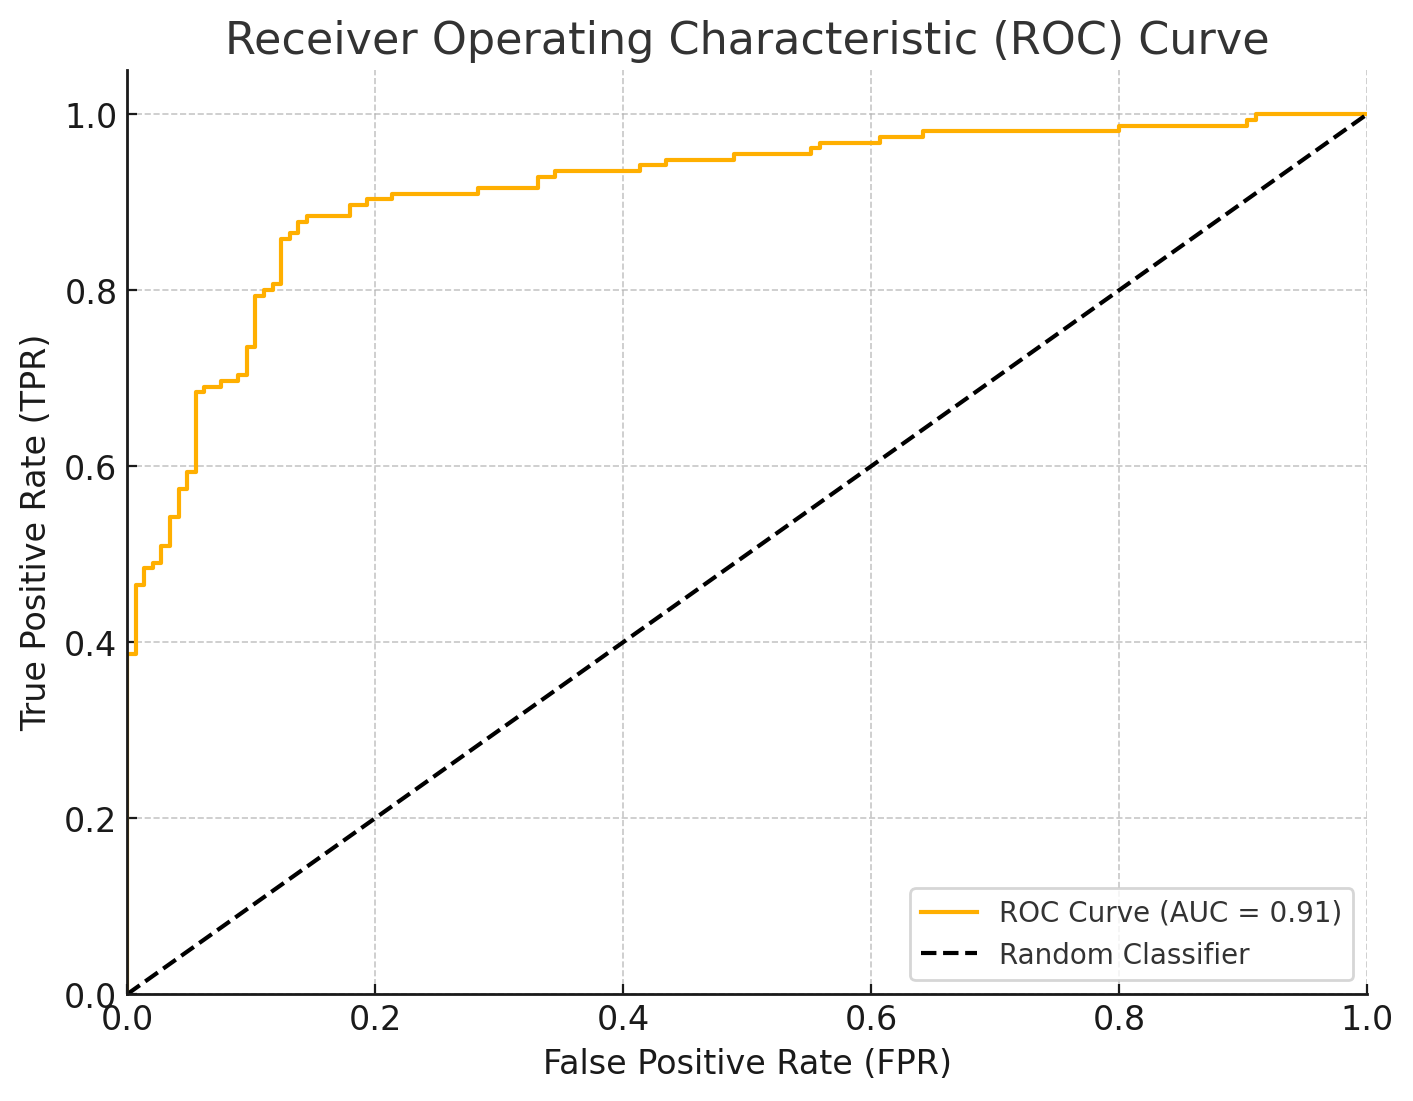
\includegraphics[width=0.7\linewidth]{img/img-receiver-operator-characteristic-curve}
			\caption{ROC curve}
			\label{fig:img-receiver-operator-characteristic-curve}
		\end{figure}
	
		The Area Under the ROC Curve (AUC) is a key indicator of model performance. The value of the AUC ranges from 0 to 1:
		
		
		\begin{itemize}
			\item A perfect classifier has an AUC of 1, indicating it achieves a TPR of 1 while keeping the FPR at 0.
			\item A model with an AUC of 0.5 performs no better than random guessing.
			\item Higher AUC values indicate better overall performance.
		\end{itemize}
		\bigskip
		
		The goal of a classifier is to maximise the TPR (correctly predicting positive instances) while minimising the FPR (incorrectly classifying negative instances as positive). Ideally, the ROC curve should approach the top-left corner of the plot, indicating a high TPR with a low FPR.
		
		In summary, the ROC curve helps to visualise and compare the trade-offs between true positives and false positives across different thresholds, and the AUC provides a single number summarising the model's ability to discriminate between positive and negative classes.
	
	
